\chapter{Технологический раздел}\label{implementation}

\section{Выбор средств программной реализации}

Для программной реализации метода была выбрана игровая среда Unity. Данный выбор обусловлен тем, что Unity предоставляет событийную модель выполнения сценариев, поддержку компонентов, механизм обработки пользовательского ввода, средства моделирования интерактивных сцен и возможность разработки логики на языке C\#~\cite{unity_monobehaviour}. Это позволяет реализовать не только сетевой обмен, но и программное обеспечение для проверки взаимодействия двух игроков.

В качестве языка программирования выбран C\#. Язык поддерживает объектно-ориентированную модель, обобщенные коллекции, перечисления, классы, интерфейсы и средства работы с сетевыми сокетами~\cite{csharp_reference}. Эти свойства используются при реализации конечных автоматов, событий, журналов неподтвержденных сообщений и сетевого транспортного уровня.

Для сетевого обмена выбран протокол UDP. Выбор UDP соответствует постановке задачи, так как метод должен работать в условиях отсутствия встроенных гарантий доставки и порядка сообщений. 
В реализации используется класс \texttt{UdpClient} пространства имен \texttt{System.Net.Sockets}, предоставляющий средства отправки и приема UDP-датаграмм~\cite{dotnet_udpclient}. 
Прикладная надежность реализуется через подтверждения, повторную отправку, контроль идентификаторов событий и проверку порядка сообщений.

\section{Структура программного обеспечения}

Разработанное программное обеспечение состоит из нескольких групп модулей:
\begin{itemize}
	\item модуль сетевого обмена;
	\item модуль синхронизации событий и конечных автоматов;
	\item модули объектов, реализующих интерфейс конечного автомата;
	\item модули пользовательского взаимодействия;
	\item модули сбора исследовательских метрик.
\end{itemize}

Основные классы программной реализации приведены в таблице~\ref{tab:implementation-modules}.

\begin{table}[H]
	\caption{Основные классы программной реализации}
	\label{tab:implementation-modules}
	\centering
	\small
	\renewcommand{\arraystretch}{1.2}
	\begin{tabular}{|p{6.2cm}|p{7.8cm}|}
		\hline
		Класс & Назначение \\ \hline
		\texttt{UdpEventTransport} & Отправка и прием UDP-сообщений, имитация потерь, задержки, вариативности задержки и дублирования пакетов \\ \hline
		\texttt{NetworkMessage} & Представление сетевого сообщения, содержащего игровое событие, подтверждение или служебное сообщение подключения \\ \hline
		\texttt{EventFsmSyncManager} & Центральный модуль синхронизации событий, обработки подтверждений, повторной отправки и применения событий к конечным автоматам \\ \hline
		\texttt{PuzzleEvent} & Представление логически значимого игрового события \\ \hline
		\texttt{IFsmPuzzleObject} & Интерфейс объектов, состояние которых изменяется через конечный автомат \\ \hline
		\texttt{PuzzleDoor} & Пример объекта, реализующего интерфейс \texttt{IFsmPuzzleObject} \\ \hline
		\texttt{ToggleBridge} & Пример объекта, реализующего интерфейс \texttt{IFsmPuzzleObject} \\ \hline
		\texttt{CoopHoldPuzzleController} & Пример объекта, реализующего интерфейс \texttt{IFsmPuzzleObject} для составного состояния взаимодействия \\ \hline
		\texttt{ColorSequenceController} & Пример объекта, реализующего интерфейс \texttt{IFsmPuzzleObject} для последовательной обработки событий \\ \hline
		\texttt{ResearchMetrics} & Сбор статистики отправки сообщений, потерь, повторных отправок, отклоненных дубликатов и примененных событий \\ \hline
	\end{tabular}
\end{table}


Структура программного обеспечения представлена в виде диаграммы классов на рисунке~\ref{img:implementation-class-diagram}. Конкретные классы игровых объектов на диаграмме рассматриваются не как самостоятельная предметная область, а как реализации общего интерфейса \texttt{IFsmPuzzleObject}, через который метод применяет подтвержденные события к конечным автоматам.

\begin{figure}[H]
	\centering
	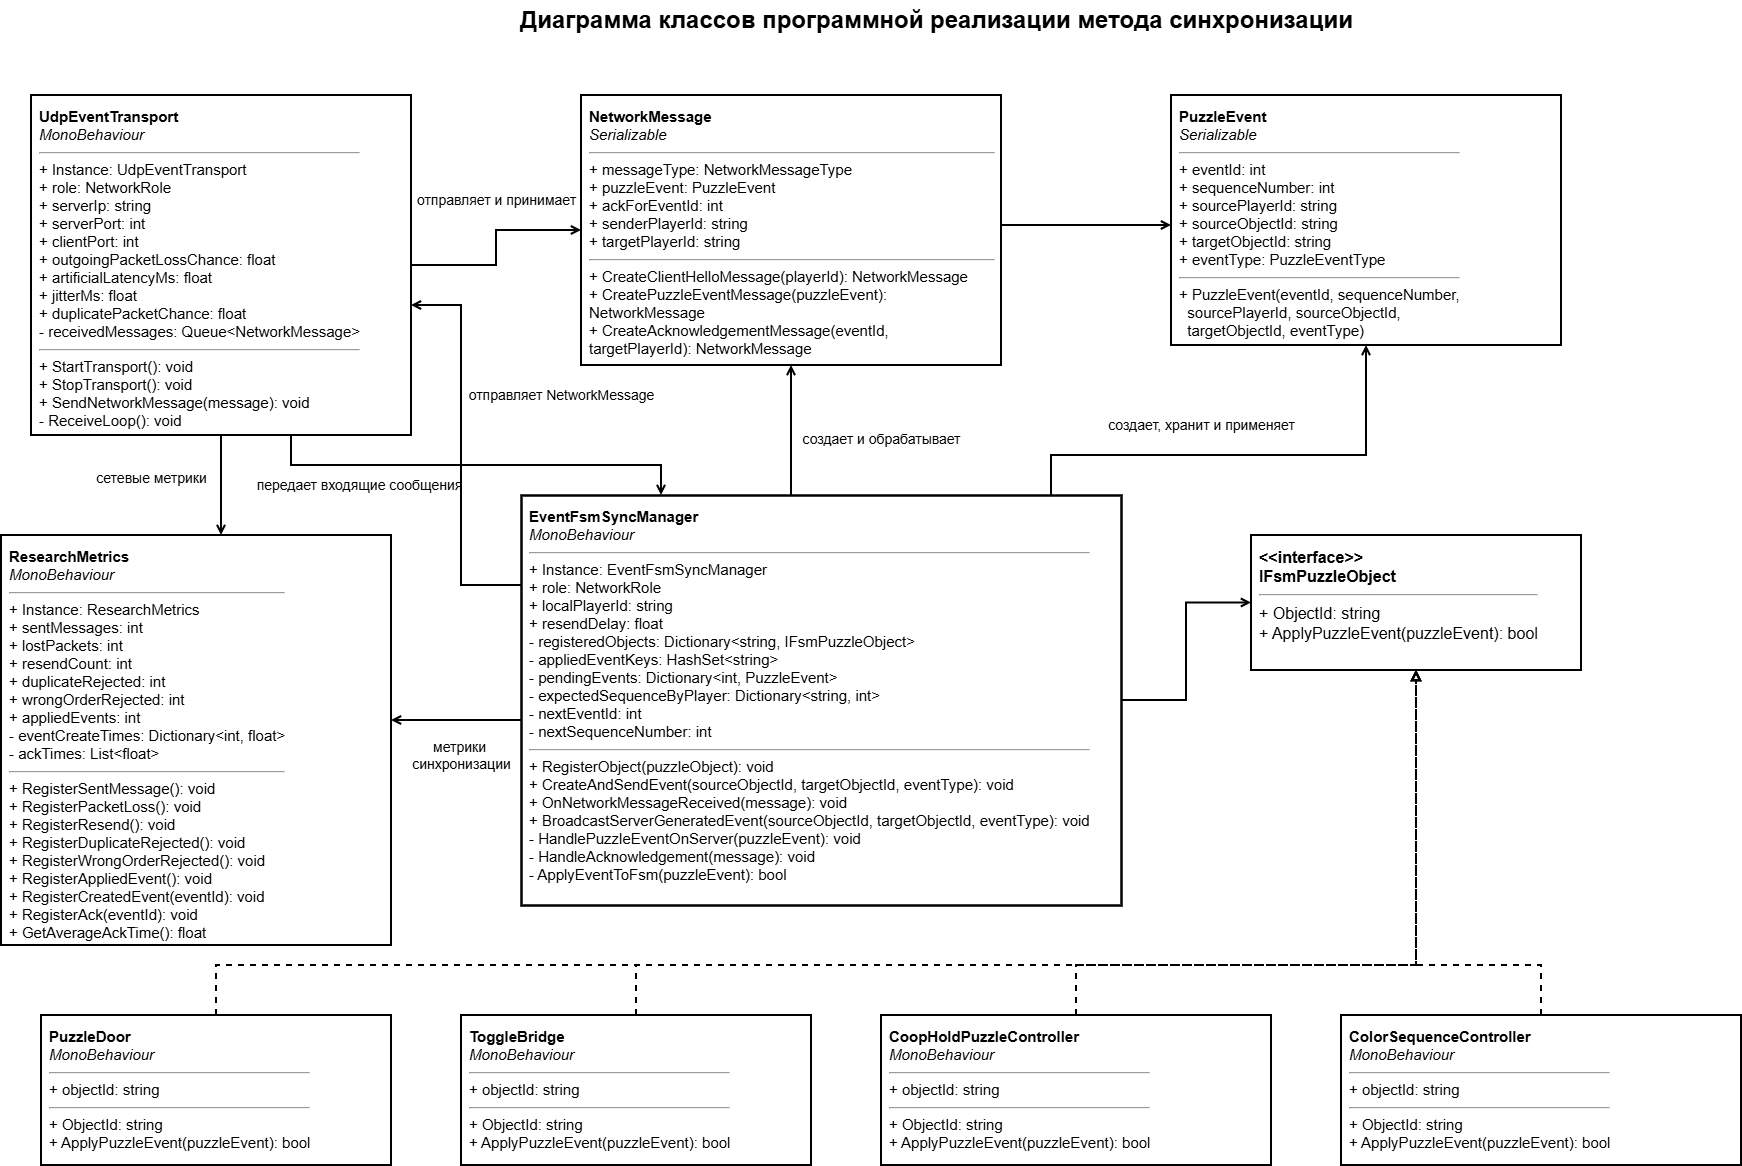
\includegraphics[width=\textwidth]{inc/img/class_diagram.png}
	\caption{Диаграмма классов программной реализации}
	\label{img:implementation-class-diagram}
\end{figure}

\section{Реализация сетевого обмена}

Сетевой обмен реализован в классе \texttt{UdpEventTransport}. Объект данного класса может работать в одной из двух ролей: \texttt{Server} или \texttt{Client}. 
Роль задается перечислением \texttt{NetworkRole}. Сервер открывает UDP-сокет на серверном порту и регистрирует адреса клиентов после получения служебного сообщения \texttt{ClientHello}. 
Клиент открывает собственный UDP-сокет, хранит адрес сервера и после запуска отправляет сообщение подключения.

При отправке сообщение типа \texttt{NetworkMessage} сериализуется в JSON-строку. Затем строка преобразуется в массив байтов и передается через UDP. Перед непосредственной отправкой применяется модель сетевых условий, включающая:
\begin{itemize}
	\item вероятность потери исходящего пакета;
	\item искусственную задержку отправки;
	\item вариативность задержки;
	\item вероятность дублирования пакета.
\end{itemize}

Прием UDP-сообщений выполняется в отдельном фоновом потоке. Это необходимо для того, чтобы ожидание входящих датаграмм не блокировало основной цикл Unity. 
Полученные сообщения помещаются в очередь \texttt{receivedMessages}. Доступ к очереди синхронизируется с помощью объекта блокировки. 
В методе \texttt{Update} сообщения извлекаются из очереди и передаются в \texttt{EventFsmSyncManager} уже в основном потоке Unity.

Игровые объекты, компоненты сцены и визуальное состояние должны изменяться из основного потока по правилам Unity. 
Поэтому фоновый поток отвечает только за сетевой прием, а изменение конечных автоматов и игровых объектов выполняется после передачи сообщения в основной цикл.

Фрагмент реализации отправки сообщения с учетом потерь, задержки, вариативности задержки и дублирования приведен в листинге~\ref{lst:udp-network-conditions}.

\sourcelisting[firstline=140,lastline=205]{../src/Networking/UdpEventTransport.cs}{Отправка UDP-сообщения с имитацией сетевых условий}{lst:udp-network-conditions}

Фрагмент приема сообщений в фоновом потоке и передачи их в основной поток Unity приведен в листинге~\ref{lst:udp-receive-loop}.

\sourcelisting[firstline=255,lastline=333]{../src/Networking/UdpEventTransport.cs}{Прием UDP-сообщений и обработка очереди в основном потоке}{lst:udp-receive-loop}

\section{Реализация структуры сетевого сообщения}

Сетевое сообщение представлено классом \texttt{NetworkMessage}. В реализации выделены три типа сообщений:
\begin{itemize}
	\item \texttt{ClientHello} --- служебное сообщение регистрации клиента;
	\item \texttt{PuzzleEvent} --- сообщение с игровым событием;
	\item \texttt{Acknowledgement} --- подтверждение обработки события.
\end{itemize}

Тип сообщения задается перечислением \texttt{NetworkMessageType}. Для создания сообщений используются статические методы:
\begin{itemize}
	\item \texttt{CreateClientHelloMessage};
	\item \texttt{CreatePuzzleEventMessage};
	\item \texttt{CreateAcknowledgementMessage}.
\end{itemize}

Игровое событие представлено классом \texttt{PuzzleEvent}. Событие содержит идентификатор, номер последовательности, идентификатор игрока-отправителя, идентификатор исходного объекта, 
идентификатор целевого объекта и тип события. Тип события задается перечислением \texttt{PuzzleEventType}.

Использование единого типа \texttt{PuzzleEvent} позволяет обрабатывать игровые события одинаковым образом независимо от того, к какому объекту сцены они относятся. Конкретная логика перехода состояния реализуется внутри целевого объекта, зарегистрированного в менеджере синхронизации.

Реализация структуры сетевого сообщения и фабричных методов создания сообщений приведена в листинге~\ref{lst:network-message}.

\sourcelisting{../src/Networking/NetworkMessage.cs}{Класс сетевого сообщения}{lst:network-message}

Структура игрового события приведена в листинге~\ref{lst:puzzle-event}.

\sourcelisting{../src/Method/PuzzleEvent.cs}{Класс игрового события}{lst:puzzle-event}

\section{Реализация менеджера синхронизации событий}

Основная логика метода реализована в классе \texttt{EventFsmSyncManager}. Данный класс выполняет следующие функции:
\begin{itemize}
	\item регистрацию объектов, реализующих интерфейс \texttt{IFsmPuzzleObject};
	\item создание локальных игровых событий;
	\item присвоение событию идентификатора и номера последовательности;
	\item отправку события через транспортный уровень;
	\item хранение неподтвержденных событий;
	\item повторную отправку события при отсутствии подтверждения;
	\item обработку входящих событий на сервере;
	\item обработку подтвержденных сервером событий на клиенте;
	\item фильтрацию дубликатов;
	\item контроль порядка событий от каждого игрока;
	\item применение события к целевому конечному автомату.
\end{itemize}

Для хранения объектов, состояние которых изменяется через конечные автоматы, используется словарь \texttt{registeredObjects}. 
Ключом является строковый идентификатор объекта, значением --- объект, реализующий интерфейс \texttt{IFsmPuzzleObject}. 
Благодаря этому сетевое событие может быть доставлено конкретному объекту по полю \texttt{targetObjectId}.

Для защиты от повторной обработки используется множество \texttt{appliedEventKeys}. Ключ события формируется из идентификатора игрока-отправителя и идентификатора события. 
Если событие с таким ключом уже было применено, повторный пакет не изменяет состояние конечного автомата.

Для реализации подтверждений используется словарь \texttt{pendingEvents}. В нем хранятся события, отправленные клиентом, но еще не подтвержденные сервером. 
После получения сообщения \texttt{Acknowledgement} соответствующее событие удаляется из словаря.

Для контроля порядка сообщений используется словарь \texttt{expectedSequenceByPlayer}. Для каждого игрока хранится номер следующего ожидаемого события. 
Если сервер получает событие с меньшим номером, оно считается устаревшим. Если получен номер больше ожидаемого, событие считается пришедшим раньше недостающих событий и не применяется.

Фрагмент создания события, присвоения идентификатора, сохранения в журнале неподтвержденных событий и запуска повторной отправки приведен в листинге~\ref{lst:create-send-event}.

\sourcelisting[firstline=91,lastline=148]{../src/Method/EventFsmSyncManager.cs}{Создание события и повторная отправка до подтверждения}{lst:create-send-event}

Фрагмент обработки события на сервере приведен в листинге~\ref{lst:server-event-handling}.

\sourcelisting[firstline=258,lastline=336]{../src/Method/EventFsmSyncManager.cs}{Проверка порядка и подтверждение события на сервере}{lst:server-event-handling}

\section{Реализация подтверждений и повторной отправки}

После создания события клиент сохраняет его в \texttt{pendingEvents}, отправляет сообщение \texttt{PuzzleEvent} и запускает корутину \texttt{ResendUntilAcknowledged}. 
Пока событие присутствует в словаре неподтвержденных событий, корутина ожидает интервал \texttt{resendDelay} и повторно отправляет то же самое событие.

Повторно отправляемое событие сохраняет исходные значения \texttt{eventId} и \texttt{sequenceNumber}. 
Это необходимо, потому что повторная отправка не должна восприниматься системой как новое игровое действие. Если получатель уже применил событие, он распознает дубликат и не изменяет состояние повторно.

Сервер после успешной проверки и применения события отправляет клиенту подтверждение. Подтверждение содержит идентификатор события и идентификатор игрока, которому оно адресовано. Клиент принимает подтверждение только в том случае, если поле \texttt{targetPlayerId} совпадает с его локальным идентификатором.

Фрагмент обработки подтверждения на стороне клиента приведен в листинге~\ref{lst:ack-handling}.

\sourcelisting[firstline=210,lastline=256]{../src/Method/EventFsmSyncManager.cs}{Обработка подтверждения и удаление события из журнала ожидания}{lst:ack-handling}

\section{Реализация объектов с конечными автоматами}

Каждый игровой объект, состояние которого изменяется через сетевое событие, реализует интерфейс \texttt{IFsmPuzzleObject}. Интерфейс содержит свойство \texttt{ObjectId} и метод \texttt{ApplyPuzzleEvent}. Такой подход позволяет отделить общий механизм сетевой синхронизации от конкретной игровой логики.

При запуске объект регистрируется в \texttt{EventFsmSyncManager} вызовом метода \texttt{RegisterObject}. Менеджер сохраняет объект в словаре \texttt{registeredObjects}, где ключом является строковый идентификатор \texttt{ObjectId}. После получения подтвержденного события менеджер находит целевой объект по полю \texttt{targetObjectId} и вызывает метод \texttt{ApplyPuzzleEvent}.

В разработанном программном обеспечении классы \texttt{PuzzleDoor}, \texttt{ToggleBridge}, \texttt{CoopHoldPuzzleController} и \texttt{ColorSequenceController} выступают как примеры объектов, 
подключаемых к методу через единый интерфейс. Их внутренняя логика может различаться, однако для алгоритма синхронизации все такие объекты не отличаются,
они предоставляют идентификатор и возвращают результат применения события. Это позволяет рассматривать конкретные игровые сценарии как заменяемые реализации целевого конечного автомата, 
не изменяющие транспортный уровень и механизм согласования состояний.

Интерфейс синхронизируемого объекта приведен в листинге~\ref{lst:fsm-interface}.

\sourcelisting{../src/Method/IFsmPuzzleObject.cs}{Интерфейс объекта с конечным автоматом}{lst:fsm-interface}

Пример реализации объекта с конечным автоматом приведен в листинге~\ref{lst:puzzle-door}.

\sourcelisting[firstline=4,lastline=65]{../src/Interactables/PuzzleDoor.cs}{Регистрация и обработка события объектом \texttt{PuzzleDoor}}{lst:puzzle-door}

\section{Реализация пользовательского взаимодействия}

Пользовательское взаимодействие реализовано через интерактивные объекты сцены. Объекты, с которыми может взаимодействовать игрок, преобразуют локальное действие в вызов \texttt{CreateAndSendEvent}.
При этом локальное действие не передается по сети напрямую, оно сначала приводится к типизированному событию \texttt{PuzzleEvent}, содержащему идентификаторы источника, цели, игрока и тип операции.

Таким образом, пользовательское действие не изменяет состояние удаленного объекта напрямую. Оно преобразуется в событие, которое проходит через общий механизм сетевой синхронизации и только после проверки применяется к целевому конечному автомату.

\section{Средства имитации сетевых ошибок}

Для проверки устойчивости метода в транспортном модуле реализованы параметры искусственного ухудшения сети:
\begin{itemize}
	\item \texttt{outgoingPacketLossChance} --- вероятность потери исходящего пакета;
	\item \texttt{artificialLatencyMs} --- средняя искусственная задержка отправки;
	\item \texttt{jitterMs} --- разброс задержки;
	\item \texttt{duplicatePacketChance} --- вероятность отправки дубликата.
\end{itemize}

Эти параметры задаются в инспекторе Unity и позволяют моделировать нестабильное сетевое соединение без изменения основного алгоритма. При имитации потери сообщение не отправляется в сеть. При имитации задержки отправка откладывается на заданное время. При имитации дубликата тот же массив байтов отправляется повторно через небольшой интервал.

Сбор статистики выполняется классом \texttt{ResearchMetrics}. Он регистрирует количество отправленных сообщений, имитированных потерь, повторных отправок, отклоненных дубликатов, событий с нарушением порядка и успешно примененных событий. Также сохраняется время создания события и время получения подтверждения, что позволяет вычислять среднее время подтверждения.

Фрагмент регистрации метрик и вычисления среднего времени подтверждения приведен в листинге~\ref{lst:research-metrics}.

\sourcelisting[firstline=34,lastline=99]{../src/Research/ResearchMetrics.cs}{Сбор исследовательских метрик}{lst:research-metrics}

\section{Тестирование разработанного программного обеспечения}

Тестирование разработанного программного обеспечения выполнялось с использованием ручных сценариев, проверяющих основные функции метода синхронизации и корректность обработки сетевых ошибок. Для каждого сценария проверялось состояние целевого конечного автомата и сообщения журнала выполнения Unity.

Основные тестовые сценарии приведены в таблице~\ref{tab:implementation-tests}.

\begin{table}[H]
	\caption{Сценарии тестирования программной реализации}
	\label{tab:implementation-tests}
	\centering
	\renewcommand{\arraystretch}{1.2}
	\begin{tabular}{|p{4cm}|p{5cm}|p{5cm}|}
		\hline
		Сценарий & Действие & Ожидаемый результат \\ \hline
		Доставка события & Игрок взаимодействует с интерактивным объектом & Создается событие, сервер применяет его к конечному автомату, клиент получает подтверждение \\ \hline
		Повторная отправка & Для исходящих пакетов задается вероятность потери & При отсутствии подтверждения событие повторно отправляется с тем же идентификатором \\ \hline
		Фильтрация дубликата & Включается вероятность дублирования пакета & Дубликат события не изменяет состояние повторно \\ \hline
		Контроль порядка & Отправляется событие с номером больше ожидаемого & Событие не применяется до восстановления порядка \\ \hline
		Недопустимое событие & Событие направляется объекту, для которого его тип не подходит & Метод \texttt{ApplyPuzzleEvent} возвращает отрицательный результат, состояние объекта не изменяется \\ \hline
		Синхронизация FSM-объекта & Оба игрока формируют события для одного синхронизируемого объекта & На обеих сторонах фиксируется одинаковое логическое состояние объекта \\ \hline
	\end{tabular}
\end{table}

Сценарии тестирования проверяют не отдельные игровые действия, а свойства метода: доставку критичного события, повторную отправку, фильтрацию дубликатов, контроль порядка и сохранение согласованного состояния конечного автомата.

\section*{Вывод}

В данном разделе был обоснован выбор Unity, языка C\# и UDP-сетевого обмена для программной реализации метода обеспечения согласованности состояний двух асинхронных игроков. Была описана структура программного обеспечения, включающая транспортный уровень, менеджер синхронизации событий, представление сетевых сообщений, интерфейс объектов с конечными автоматами и средства сбора статистики.

Были рассмотрены детали реализации прикладной надежности поверх UDP, такие как подтверждение обработки события, хранение неподтвержденных событий, повторная отправка, фильтрация дубликатов и контроль порядка сообщений. 
Также был описан способ подключения объектов, реализующих интерфейс \texttt{IFsmPuzzleObject}, и сценарии тестирования разработанного программного обеспечения.
